\chapter{アニメーションの基本}
\label{chap:animation-basics}

この章では、図形を少しずつ動かしてアニメーションを作る方法を学びます。これまでの章では、1枚の静止した絵を描くことが中心でした。ここからは、\texttt{draw}が繰り返し実行される仕組みを使い、変数の値を少しずつ変えながら動きを作ります。

\section{この章の概要}

アニメーションは、少しずつ違う絵を連続して表示することで作られます。p5.jsでは、\texttt{draw}関数に書いた処理が何度も実行されます。
そのたびに位置を表す変数を少し変えると、図形が動いて見えます。

この章で扱う主な内容は次の通りです。

\begin{itemize}
    \item \texttt{setup}と\texttt{draw}の役割
    \item 位置を表す変数を少しずつ変える方法
    \item 速度を変数として扱う方法
    \item \texttt{background}を書く位置による見え方の違い
    \item \texttt{p.frameCount}によるフレーム数の利用
    \item 第4章の\texttt{arc}を動かす例
\end{itemize}

\section{setupとdraw}

p5.jsでは、\texttt{setup}関数に書いた処理は最初に一度だけ実行されます。
一方、\texttt{draw}関数に書いた処理は、プログラムが動いている間、何度も繰り返し実行されます\footnote{通常、\texttt{draw}関数は、1秒間に60回程度実行されます}。
instance modeでは、\texttt{p.setup = (): void => \{ ... \};}と\texttt{p.draw = (): void => \{ ... \};}の形で、p5.jsが実行する関数を登録します。

\begin{figure}[htbp]
    \centering
    \begin{tikzpicture}[x=1cm, y=1cm, font=\small]
        \tikzset{
            startstop/.style={
                draw=black!60,
                fill=gray!10,
                rounded corners=8pt,
                minimum width=3.2cm,
                minimum height=0.8cm,
                align=center
            },
            process/.style={
                draw=black!60,
                fill=blue!8,
                rounded corners=2pt,
                minimum width=4.0cm,
                minimum height=0.9cm,
                align=center
            },
            repeatprocess/.style={
                draw=black!60,
                fill=orange!12,
                rounded corners=2pt,
                minimum width=4.0cm,
                minimum height=0.9cm,
                align=center
            },
            arrow/.style={->, line width=0.8pt, draw=black!70},
            looparrow/.style={->, line width=0.8pt, draw=orange!80!black}
        }

        \node[startstop] (start) at (0, 0) {プログラム開始};
        \node[process] (setup) at (0, -1.5) {\texttt{p.setup}\\最初に1回だけ実行};
        \node[repeatprocess] (draw) at (0, -3.0) {\texttt{p.draw}\\何度も繰り返し実行};
        \node[process] (frame) at (0, -4.5) {画面に1枚の絵を表示\\次のフレームへ};

        \draw[arrow] (start) -- (setup);
        \draw[arrow] (setup) -- (draw);
        \draw[arrow] (draw) -- (frame);
        \draw[looparrow]
            (frame.east) -- (3.0, -4.5) -- (3.0, -3.0) -- (draw.east);

        \node[align=left, anchor=west] at (3.25, -3.75)
            {\texttt{draw}の中では\\位置や色などを\\少しずつ変えられる};
    \end{tikzpicture}
    \caption{\texttt{setup}と\texttt{draw}が実行される流れ}
    \label{fig:chapter05-setup-draw-flow}
\end{figure}

\begin{listing}[htbp]
\inputminted{ts}{listings/chapter05/setup-draw-basic.ts}
\caption{setupとdrawを使った基本形}
\label{lst:chapter05-setup-draw-basic}
\end{listing}

このサンプルでは、円の位置は変わりません。それでも\texttt{draw}関数の中身は繰り返し実行されています。今は同じ絵を何度も描いているため、静止して見えます。

\section{位置を少しずつ変える}

図形を動かすには、位置を表す変数を用意し、\texttt{draw}が実行されるたびにその値を少しずつ変えます。右に動かしたい場合は、$x$ 座標を少しずつ大きくします。

\begin{listing}[htbp]
\inputminted{ts}{listings/chapter05/moving-circle.ts}
\caption{x座標を変えて円を動かす}
\label{lst:chapter05-moving-circle}
\end{listing}

\texttt{circleX}は円の中心の $x$ 座標です。\texttt{circleSpeed}は、1回の\texttt{draw}でどれだけ右に進むかを表しています。
\[
\texttt{circleX} = \texttt{circleX} + \texttt{circleSpeed};
\]
によって、円の位置が少しずつ右へ移動します。

\begin{figure}[htbp]
    \centering
    \begin{tikzpicture}[font=\small]
        \foreach \start/\position/\value/\frameNumber in {
            0/0.65/60/1,
            3.45/0.95/62/2,
            6.90/1.25/64/3,
            10.35/1.55/66/4
        } {
            \draw[thick, fill=gray!6]
                (\start,0) rectangle +(2.65,-1.8);
            \filldraw[fill=orange!45, draw=black]
                (\start+\position,-0.9) circle (0.28);
            \node[align=center] at (\start+1.325,-2.25)
                {\frameNumber 回目の\texttt{draw}\\
                 \texttt{circleX = \value}};
        }

        \draw[->, thick] (2.72,-0.9) -- (3.35,-0.9)
            node[midway, above, font=\scriptsize]{\texttt{+2}};
        \draw[->, thick] (6.17,-0.9) -- (6.80,-0.9)
            node[midway, above, font=\scriptsize]{\texttt{+2}};
        \draw[->, thick] (9.62,-0.9) -- (10.25,-0.9)
            node[midway, above, font=\scriptsize]{\texttt{+2}};
    \end{tikzpicture}
    \caption{\texttt{draw}のたびにx座標が変わって円が移動する様子}
    \label{fig:chapter05-circle-frame-sequence}
\end{figure}

図\ref{fig:chapter05-circle-frame-sequence}では、4回の\texttt{draw}を別々の絵として並べています。サンプルと同じように、\texttt{circleX}へ毎回\texttt{2}を加えています。図では変化を見分けやすくするため、円の移動距離を実際の比率より大きく表しています。実際のブラウザでは、この描画が短い間隔で続けて表示されるため、円がなめらかに右へ動いているように見えます。

\begin{pointbox}{動きの基本}
アニメーションの基本は、「描く」「値を変える」を繰り返すことです。位置を変えれば移動し、大きさを変えれば拡大や縮小のように見えます。
\end{pointbox}

\section{実数の速度を使う}

速度の値を小さくすると、動きはゆっくりになります。TypeScriptの\texttt{number}型には\texttt{2}と\texttt{0.5}のどちらも保存できるため、\texttt{0.8}のような値を速度として使うことができます。

\begin{listing}[htbp]
\inputminted{ts}{listings/chapter05/fractional-speed.ts}
\caption{小数の速度で円をゆっくり動かす}
\label{lst:chapter05-fractional-speed}
\end{listing}

このサンプルでは、\texttt{circleY}を少しずつ大きくしています。p5.jsでは下に進むほど $y$ 座標が大きくなるため、円は下へ移動します。

\section{backgroundをdrawに書く}

アニメーションでは、前のフレームに描いた図形を消してから、新しい位置に図形を描くことがよくあります。そのためには、\texttt{background}関数を\texttt{draw}関数の中に書きます。

\begin{listing}[htbp]
\inputminted{ts}{listings/chapter05/background-in-draw.ts}
\caption{drawの中で背景を塗り直す}
\label{lst:chapter05-background-in-draw}
\end{listing}

このサンプルでは、毎回\texttt{p.background(245)}で画面全体を塗り直してから円を描いています。そのため、前の位置の円は残らず、1つの円が動いているように見えます。

\section{backgroundをsetupに書く}

\texttt{background}関数を\texttt{setup}関数にだけ書くと、背景は最初に一度だけ塗られます。その後の\texttt{draw}では前の図形が消されないため、動いた跡が残ります。

\begin{listing}[htbp]
\inputminted{ts}{listings/chapter05/background-in-setup.ts}
\caption{setupだけで背景を塗る}
\label{lst:chapter05-background-in-setup}
\end{listing}

このサンプルでは、円が移動した場所が画面に残ります。これは間違いとは限りません。軌跡を描きたいときには便利です。ただし、1つの物体だけが動いているように見せたい場合は、\texttt{background}を\texttt{draw}の中に書きます。

\begin{figure}[htbp]
    \centering
    \begin{minipage}[t]{0.47\linewidth}
        \centering
        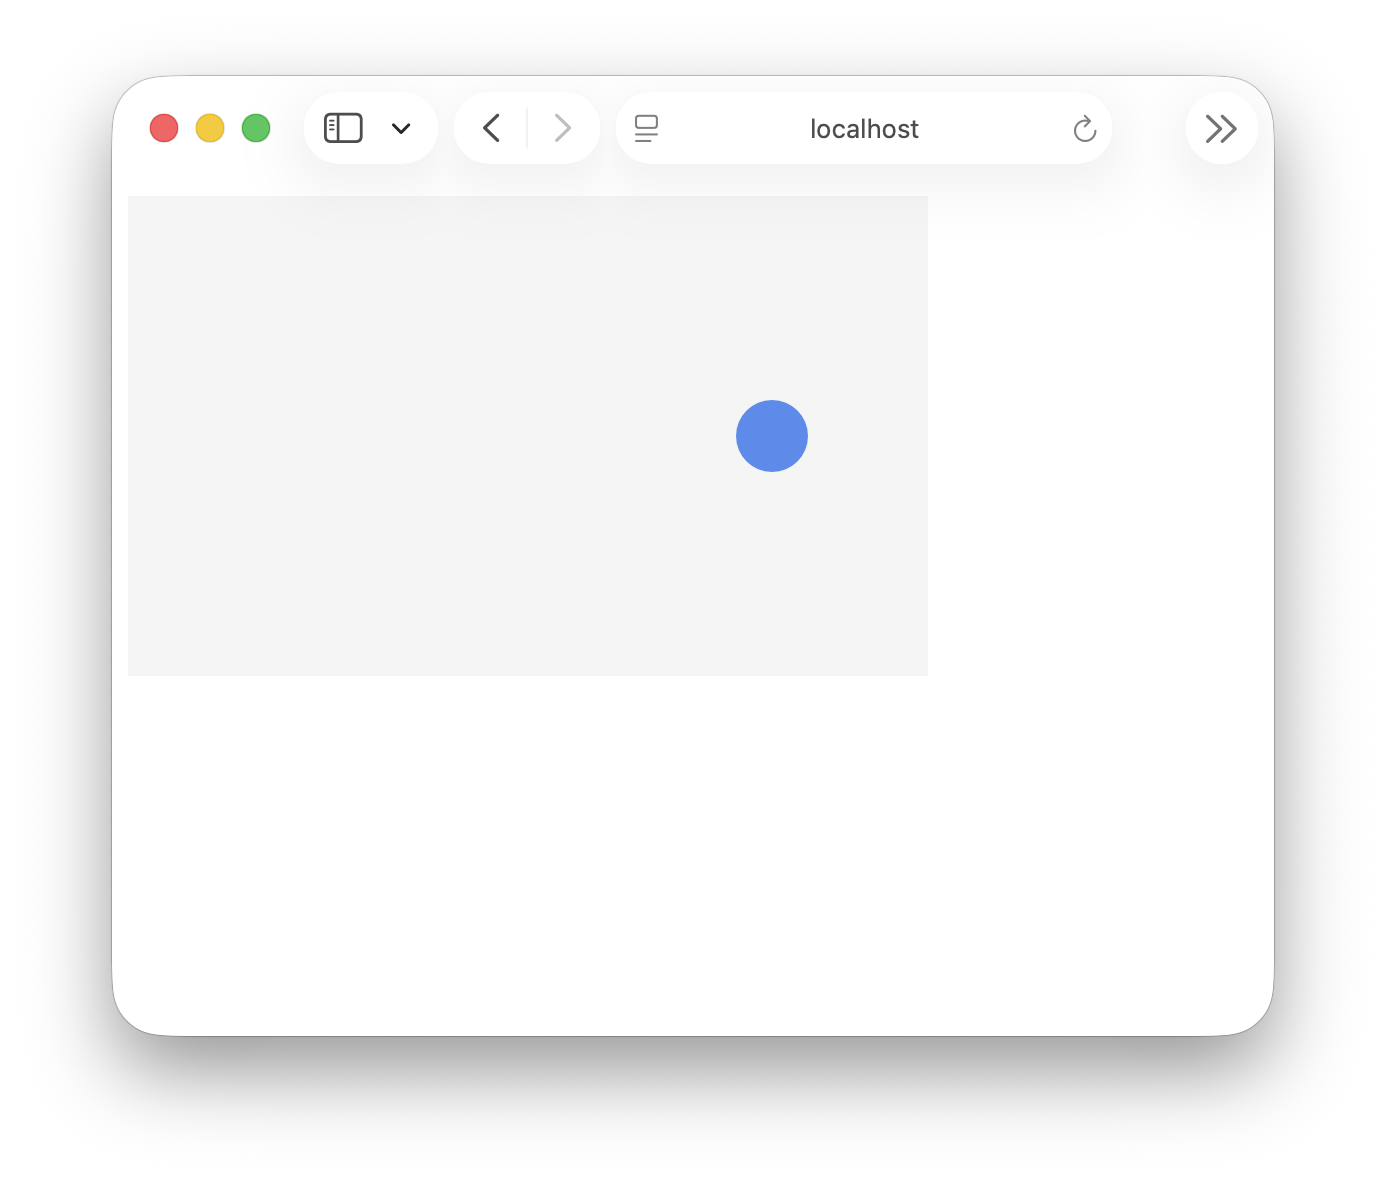
\includegraphics[
            width=\linewidth,
            trim=50 212 193 35,
            clip
        ]{figures/chapter05/background-in-draw.png}

        \small \texttt{draw}で\texttt{background}を実行
    \end{minipage}
    \hfill
    \begin{minipage}[t]{0.47\linewidth}
        \centering
        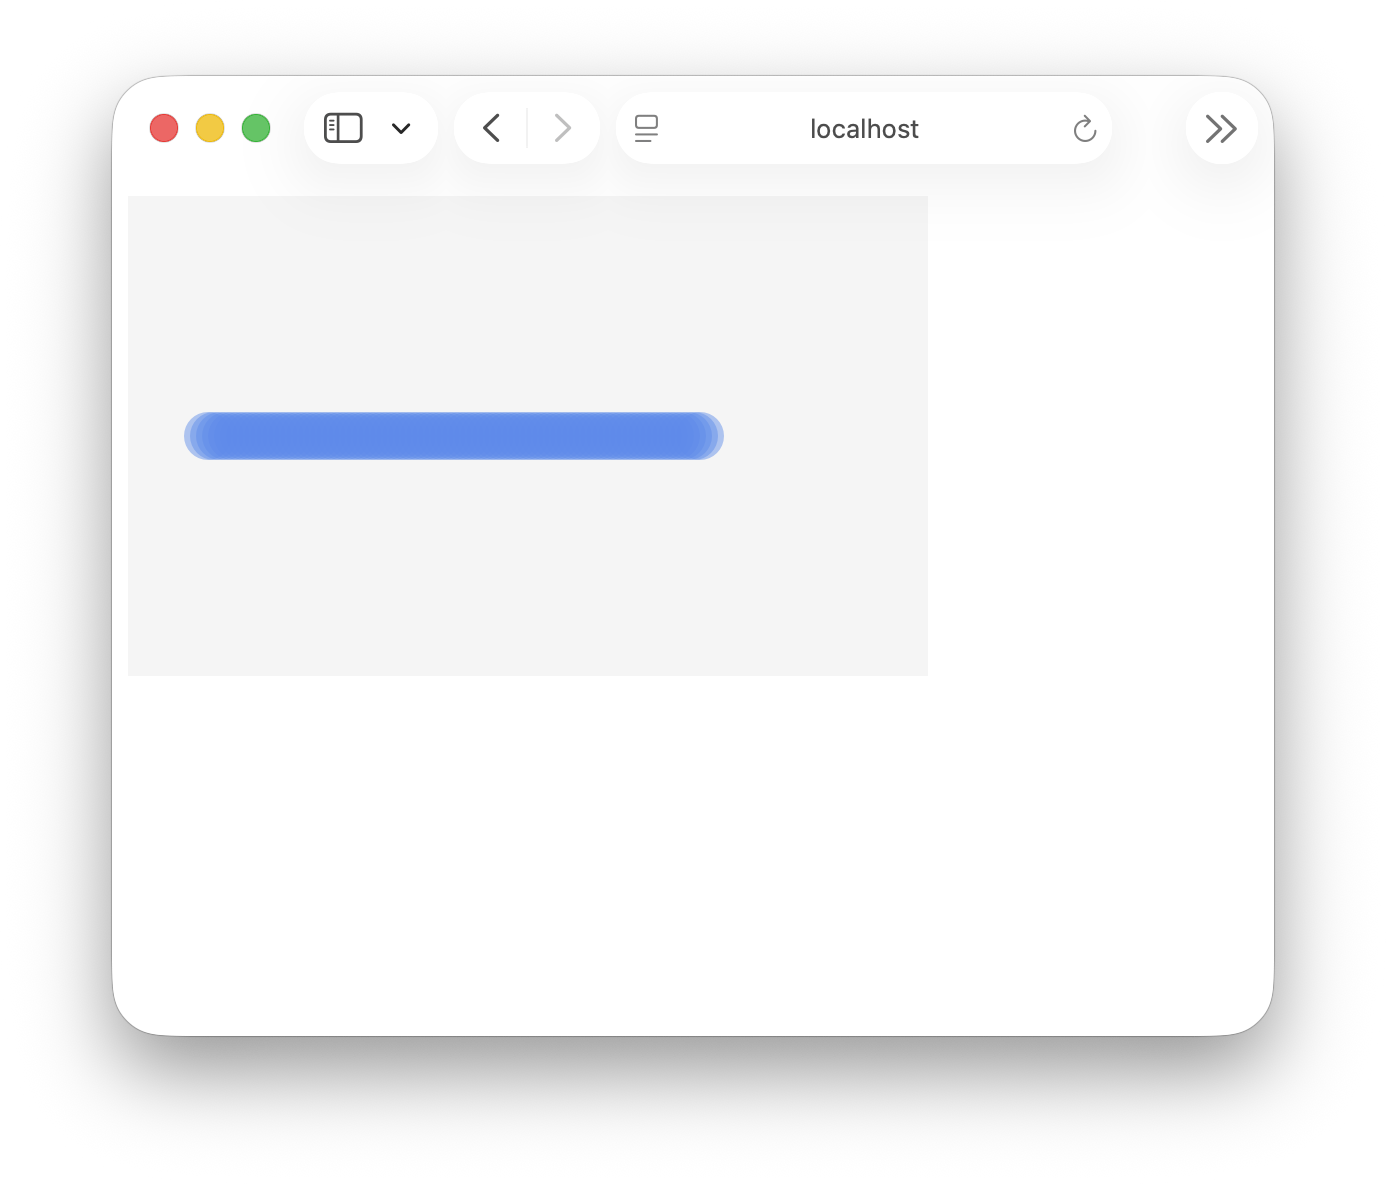
\includegraphics[
            width=\linewidth,
            trim=50 212 193 35,
            clip
        ]{figures/chapter05/background-in-setup.png}

        \small \texttt{setup}で最初にだけ\texttt{background}を実行
    \end{minipage}
    \caption{\texttt{background}を書く場所による実行画面の違い}
    \label{fig:chapter05-background-placement-results}
\end{figure}

図\ref{fig:chapter05-background-placement-results}の左側では、\texttt{draw}のたびに背景を塗り直すため、現在の位置にある円だけが見えます。右側では、背景を最初に一度しか塗らないため、それまでに描かれた円が軌跡として残ります。

\begin{notebox}{backgroundの場所}
\texttt{background}を\texttt{draw}に書くと毎回画面を消します。\texttt{setup}にだけ書くと、前に描いた図形が残ります。どちらが正しいかではなく、作りたい見た目に合わせて選びます。
\end{notebox}

\section{\texttt{frameCount}を使う}

p5.jsには、システム変数\texttt{frameCount}が用意されています。
これは、\texttt{draw}が何回実行されたかを表す数値です。
毎回少しずつ増える値として使うことができます。
コード上では、\texttt{p.frameCount}のように、スケッチを表す変数を通して使います。

\begin{listing}[htbp]
\inputminted{ts}{listings/chapter05/frame-count.ts}
\caption{frameCountで大きさを変える}
\label{lst:chapter05-frame-count}
\end{listing}

このサンプルでは、\texttt{frameCount}変数を使って円の直径を計算しています。時間が進むにつれて\texttt{frameCount}変数の値が大きくなるため、円も少しずつ大きくなります。

\begin{notebox}{frameCountは読み取る値}
\texttt{frameCount}変数はp5.jsが用意している値です。自分で代入して変更するものではなく、現在のフレーム数を読み取るために使います。
\end{notebox}

\section{arcを動かす}

第4章では、\texttt{arc}関数を使って口が開いた円を描きました(サンプル\ref{lst:chapter04-arc-pacman})。
同じ考え方で、\texttt{arc}の中心座標を少しずつ変えると、パックマン風のキャラクターが移動しているように見せることができます。

\begin{listing}[htbp]
\inputminted[fontsize=\small]{ts}{listings/chapter05/moving-pacman.ts}
\caption{arcで描いたキャラクターを動かす}
\label{lst:chapter05-moving-pacman}
\end{listing}

このサンプルでは、\texttt{characterX}を少しずつ大きくしています。\texttt{arc}関数の中心を表す引数の $x$ 座標に\texttt{characterX}を使っているため、キャラクター全体が右へ移動します。

\begin{pointbox}{p.を付ける理由}
instance modeでは、p5.jsが用意している命令や値を\texttt{p}から使います。そのため、\texttt{background}ではなく\texttt{p.background}、\texttt{frameCount}ではなく\texttt{p.frameCount}と書きます。
\end{pointbox}

\section{よくある間違い}

アニメーションでは、文法は正しくても、変数を更新する場所や背景を塗る場所によって、思った通りに見えないことがあります。

\begin{mistakebox}{位置を表す変数をdrawの中で毎回初期化する}
\texttt{draw}の中で\texttt{let circleX: number = 60;}のように書くと、毎回同じ値から始まってしまいます。動かしたい位置の変数は、\texttt{draw}の外側に用意します。
\end{mistakebox}

\begin{mistakebox}{変数の値を更新していない}
円を描くだけでは位置は変わりません。\texttt{circleX = circleX + circleSpeed;}のように、位置を表す変数を更新する必要があります。
\end{mistakebox}

\begin{mistakebox}{backgroundの場所を間違える}
前の図形を消したいときは、\texttt{p.background}を\texttt{p.draw}の中に書きます。軌跡を残したいときは、\texttt{p.setup}だけに書く方法もあります。
\end{mistakebox}

\begin{mistakebox}{速さを大きくしすぎる}
\texttt{circleSpeed}が大きすぎると、図形が一気に移動して見えます。最初は\texttt{1}から\texttt{3}くらいの値で試すと違いが分かりやすいです。
\end{mistakebox}

\section{まとめ}

この章では、\texttt{setup}と\texttt{draw}を使ってアニメーションを作る基本を学びました。\texttt{setup}は最初に一度だけ実行され、\texttt{draw}は繰り返し実行されます。

また、位置や速度を変数で表し、\texttt{draw}の中で少しずつ値を変えることで動きを作りました。\texttt{background}を書く場所によって、前の絵を消すか、軌跡として残すかが変わることも確認しました。

\section{演習問題}

この章の演習では、円や\texttt{arc}を少しずつ動かしながら、アニメーションの基本を確認します。まずは数値を変えて動きの違いを観察し、最後は自分の動く作品を作ってみましょう。

\begin{enumerate}
    \item \texttt{moving-circle.ts}の\texttt{circleSpeed}を変えて、円の速さを変えてください。
    \item \texttt{circleX}の初期値を変えて、円が動き始める位置を変えてください。
    \item \texttt{circleY}を変化させて、円が下に動くアニメーションを作ってください。
    \item \texttt{circleSpeed}に小数を使い、ゆっくり動く円を作ってください。
    \item \texttt{background}関数を\texttt{draw}から\texttt{setup}へ移動し、見え方の違いを説明してください。
    \item \texttt{background}関数の色を変えて、暗い背景や明るい背景で動きを確認してください。
    \item \texttt{frameCount}変数を使い、時間とともに円が大きくなるサンプルを変更してください。
    \item \texttt{arc}関数で描いたキャラクターの大きさや色を変えてください。
    \item \texttt{characterSpeed}を変えて、パックマン風のキャラクターの移動速度を調整してください。
    \item 挑戦問題として、円、四角形、\texttt{arc}のいずれかを使い、横または縦に動く短いアニメーション作品を作ってください。
\end{enumerate}
